\insertmeeting 
	{Car Drive} 
	{09/24/22}
	{Hagerty High School}
	{Nathan, Ritam, Robert}
	{Images/RobotPics/robot.jpg}
	{1:30 - 3:30}
	
\hhscommittee{Hardware}
\noindent\hfil\rule{\textwidth}{.4pt}\hfil
\subsubsection*{Goals}
\begin{itemize}
    \item Create a more solid plan for the tricycle drive
	\item Improve stability of the drivetrain


\end{itemize} 

\noindent\hfil\rule{\textwidth}{.4pt}\hfil

\subsubsection*{Accomplishments}
After deciding to move forward with the tricycle drive while developing a backup mecanum drive we split up into groups to tackle each of these designs. Today, the members wanting to work on the tricycle design met to discuss some of its issues, how to fix them, and what this year's drivetrain should look like. The main issue with a tricycle design, which is particularly pronounced in this game is its relative instability. Because the tricycle is supported by only 3 wheels instead of 4, the center of mass must say over a smaller area than a tank drive of a similar size. (figure 1) We figure that this will be a larger problem than it was last year, because of the height robots must reach to score on the tallest junction. Because this problem was an inherent flaw of a tricycle design, we were struggling to come up with any good solutions. Feeling a bit cornered, we broke down the idea into two fundamental questions: why did the tricycle design work while testing and why will it potentially not work? To start with, we answered the first question, saying that the design had worked not because it had three wheels as the name suggests, but because of its front wheel steering. The benefits of the design, maintaining speed through corners and giving the driver more control while turning, had nothing to do with the robot’s number of wheels. Moving on to the second fundamental question, we discussed that the tricycle design might not work because of the triangular shape of its base, caused by having only three points of contact with the ground. This problem is directly related to the robot’s number of wheels. Realizing this, we came to the conclusion that what we wanted wasn’t a tricycle drive, but a front-wheel steering drivetrain. To get the most out of our design, we came up with the idea of adding a wheel to the tricycle design, allowing it to steer with its front wheel while also having a base defined by 4  points, increasing its area and making the robot much more stable. What resulted from this is a design that resembles a car, with its 2 front wheels turning to control the steering and its 2 back wheels powered by motors causing the robot to move.


\begin{figure}[ht]
\centering
\begin{minipage}[b]{.48\textwidth}
  \centering
  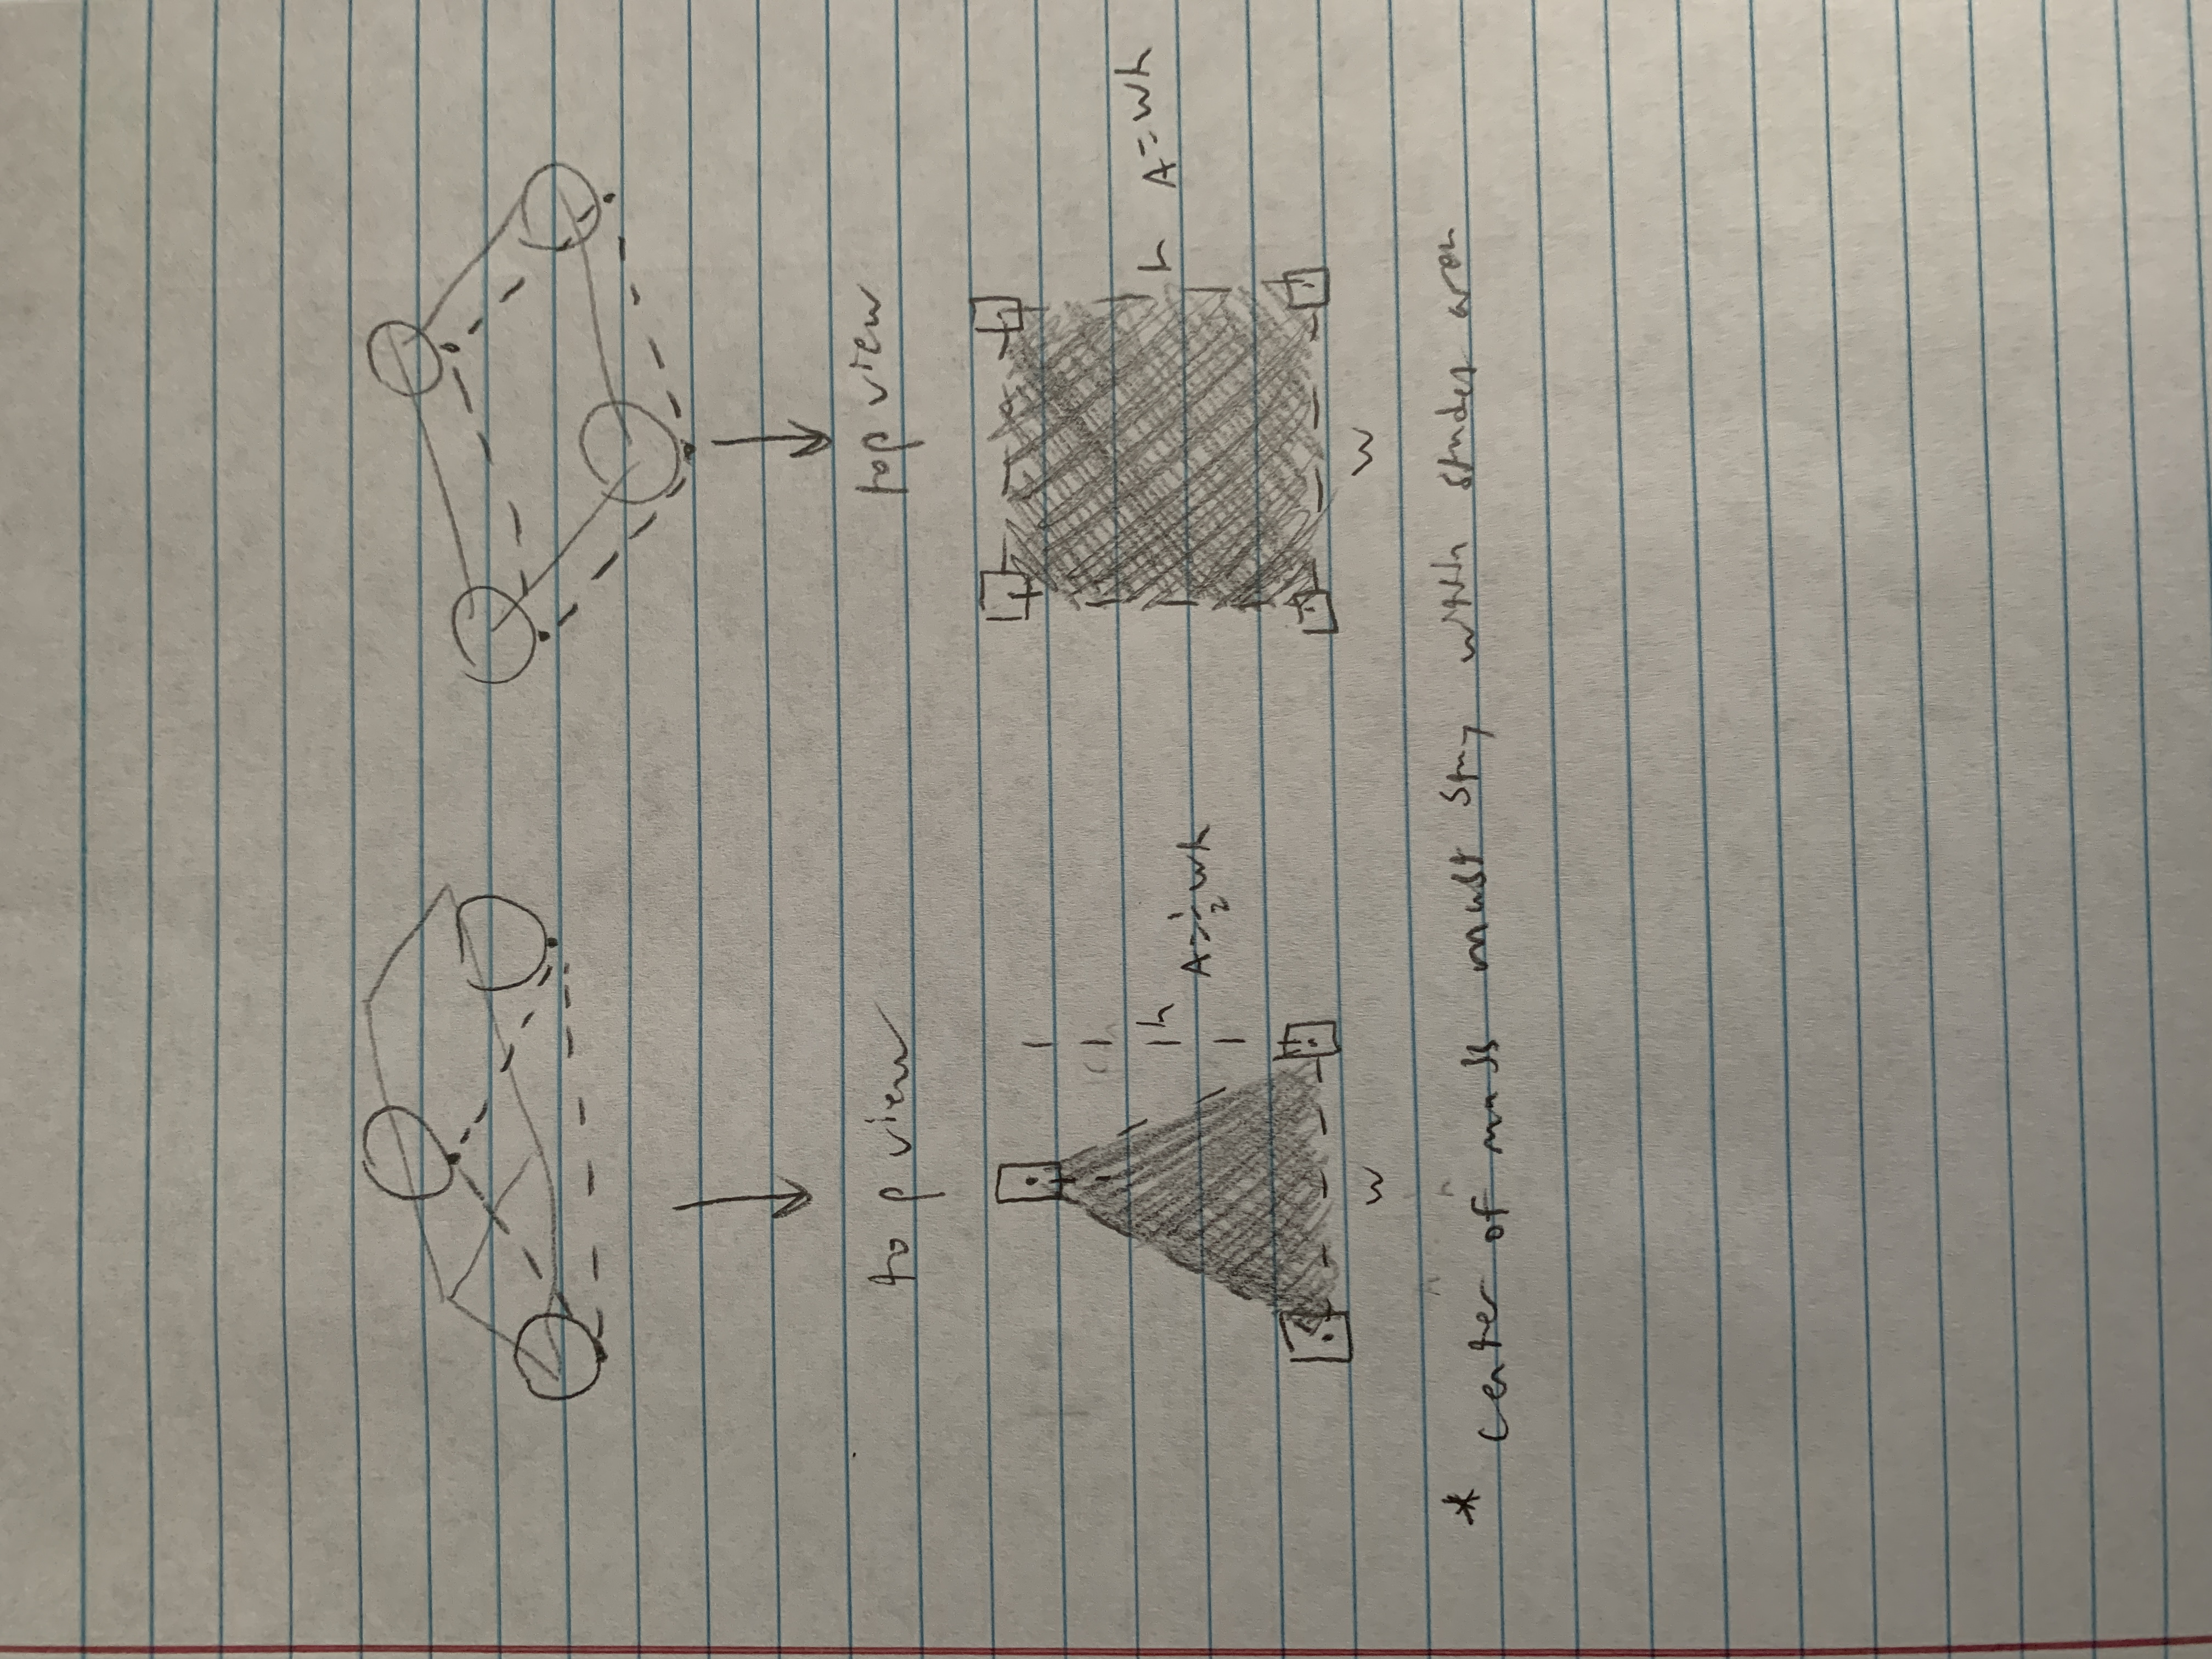
\includegraphics[width=0.95\textwidth]{Meetings/September/09-24-22/9-24-22_Hardware_Figure1.JPG}
  \caption{Diagram of car drive}
  \label{fig:pic1}
\end{minipage}%
\hfill%
\begin{minipage}[b]{.48\textwidth}
  \centering
  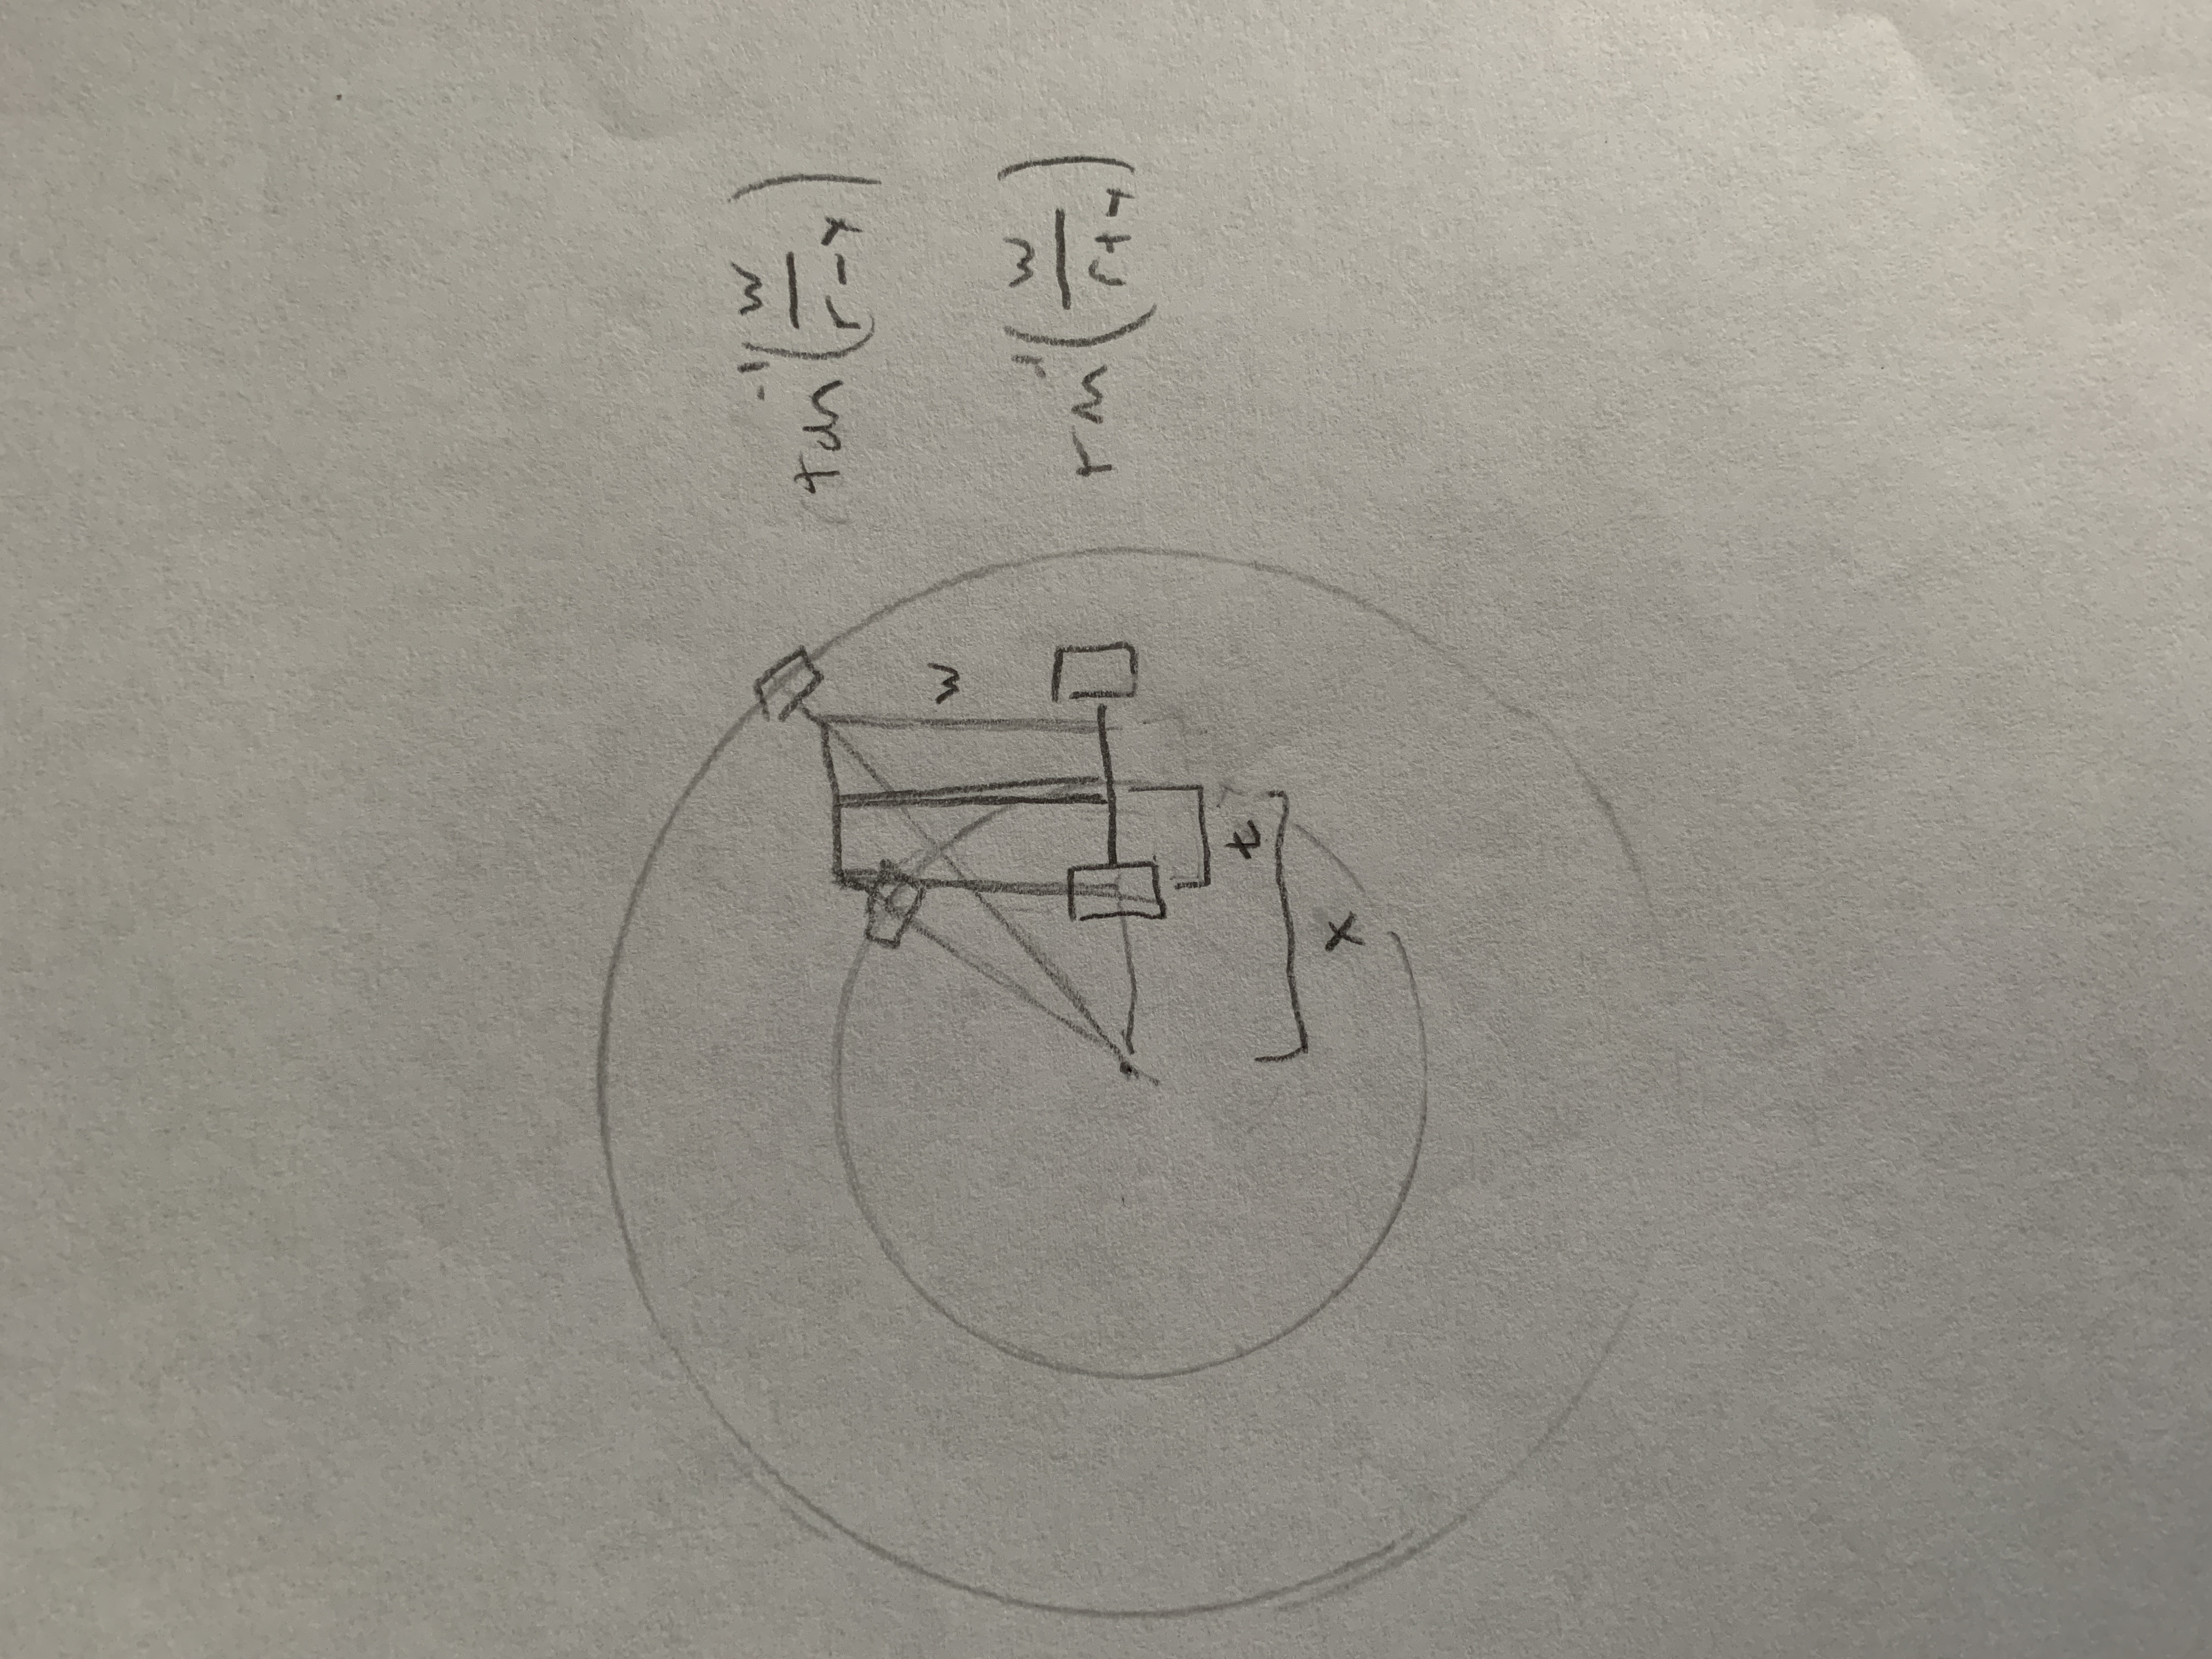
\includegraphics[width=0.95\textwidth]{Meetings/September/09-24-22/9-24-22_Hardware_Figure2.JPG}
  \caption{Math of car drive}
  \label{fig:pic2}
\end{minipage}
\end{figure}

% \begin{figure}[htp]
% \centering
% 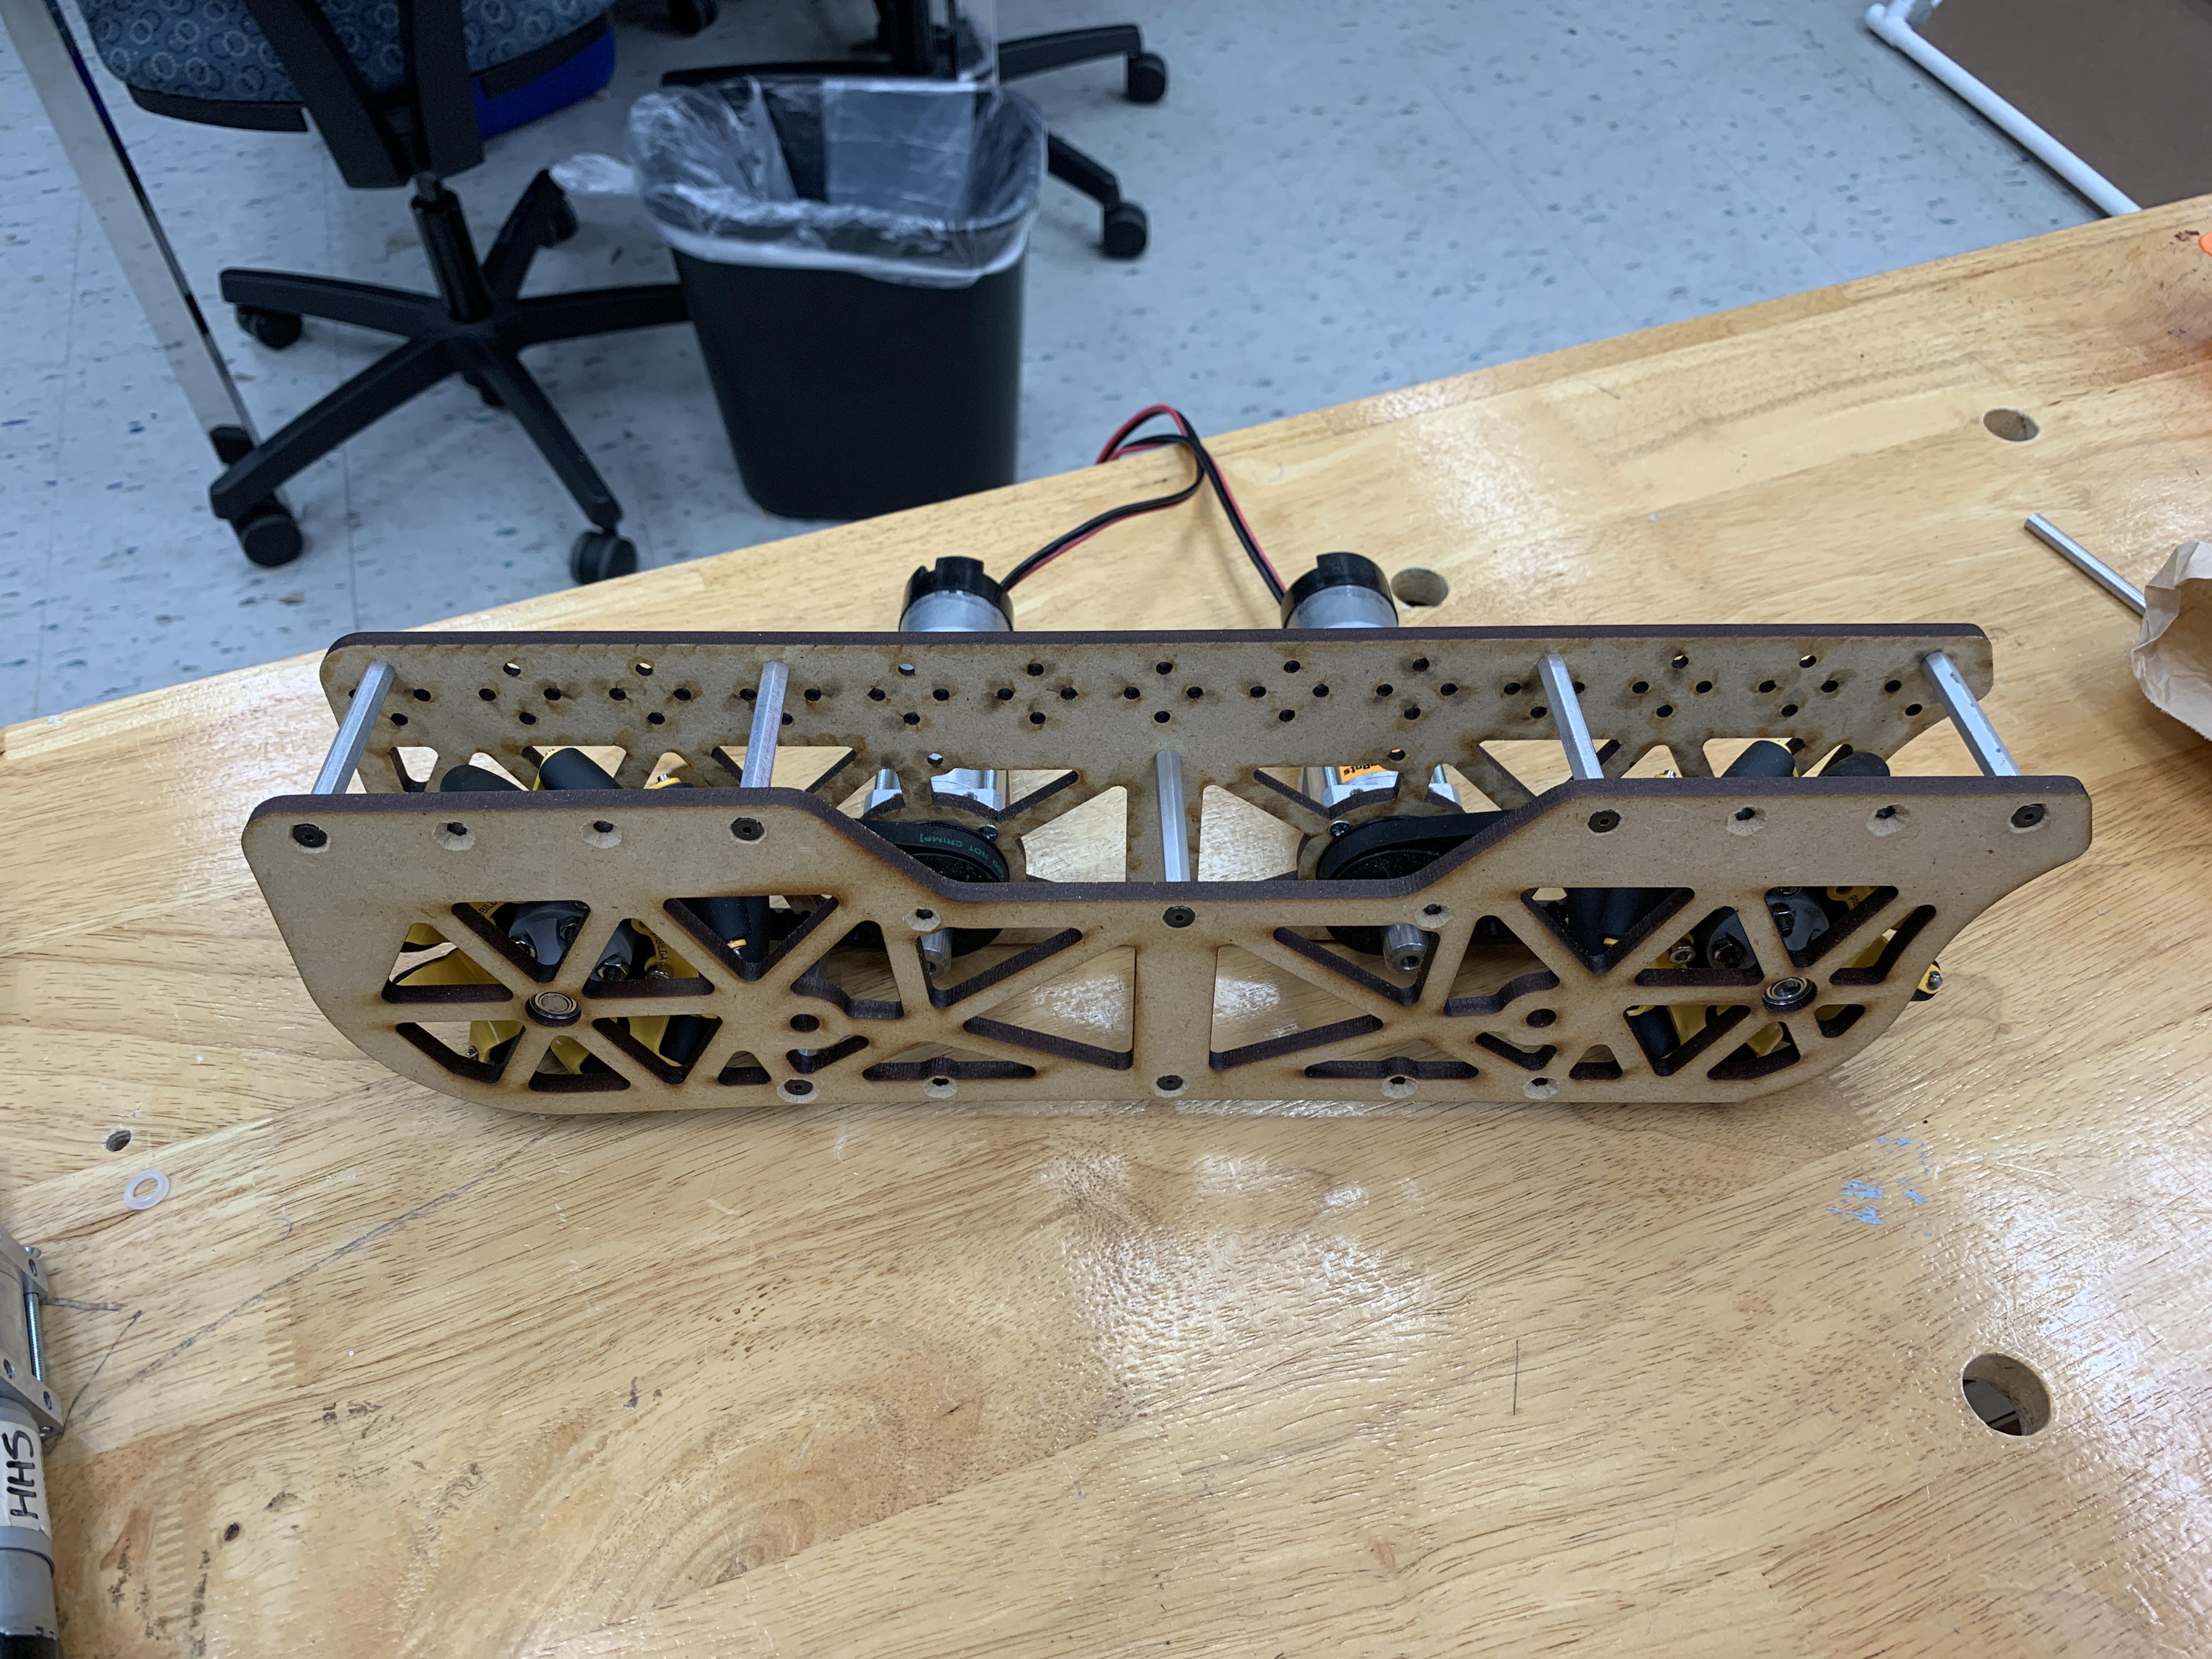
\includegraphics[width=0.9\textwidth, angle=0]{Meetings/July/07-21-21/drivetrain_7-20-21-NathanForrer.jpg}
% \caption{First half of the drivetrain.}
% \label{fig:072121_1}
% \end{figure}

\whatsnext{
\begin{itemize}
    \item CAD four bar intake
    
\end{itemize} 
}
